\documentclass[aspectratio=1610, 10pt]{beamer}
\usepackage{tikz}
\PassOptionsToPackage{height=1.2cm}{beamerouterthemesidebar}

% Theme
\usetheme{LMS} % LMPS inspired


% packages 
\usecolortheme{default}
\usepackage{xcolor}
\usepackage{multicol}
\usepackage{multirow}
\newcommand\hmmax{0}
\newcommand\bmmax{0}
\usepackage{soul}
\usepackage{animate}

% Nested delimiters (parenthesis) (https://tex.stackexchange.com/questions/36039/automatic-size-adjustment-for-n    ested-parentheses)
\delimitershortfall=-1pt
\def\doubleunderline#1{\underline{\underline{#1}}}

% My notations
\usepackage{MyPresNotations}
\usefonttheme[onlymath]{serif}% Serif for math font
\usepackage{verbatim}
\usepackage{listings}
\captionsetup{labelformat=empty,labelsep=none} 

\newcommand{\inputTikZ}[2]{%  
	\scalebox{#1}{\input{#2}}  
}


% \author[\textcolor{white!70!black}{Katka \& Alexandre}]{\textcolor{BleuLMS}{Katerina Skardova \& Alexandre Daby-Seesaram}} % (optional)

% \title[ANR \\ MLQ-CT] %optional
% {\bfseries \textcolor{BleuLMS}{Surrogate Methods for Patient-Specific Lung Modelling}
% }
% \subtitle{\itshape\textcolor{GreenLMS}{ANR MLQ-CT}}


\author[\textcolor{white!70!black}{Katka \& Alexandre}]{\textcolor{BleuLMS!10}{Katerina Skardova \& Alexandre Daby-Seesaram}} % (optional)

\title[ANR \\ MLQ-CT] %optional
{\bfseries \textcolor{BleuLMS!10}{Surrogate Methods for Patient-Specific Lung Modelling}
}
\subtitle{\itshape\textcolor{GreenLMS!10}{ANR MLQ-CT}}


% What about : 
% A: Perfect !
% Surrogate Modelling for Patient-Specific Parameterized Lung Simulations
% or: Surrogate Methods for Patient-Specific Lung Modeling
% A : yes the scond one is even better !
% Cool

\date[VLC 2023] % (optional)
{\textcolor{BleuLMS!10}{12$^{\text{th}}$ of February 2024}}



\begin{document}
	%	
			{
%			\setbeamertemplate{background canvas}{bg=accentcolor}
			\setbeamertemplate{sidebar canvas left}{}
			\setbeamertemplate{sidebar left}{}
			\setbeamertemplate{background} 
			{	\hspace*{\sidebarwidth}
				\hspace{-1.9cm}
				
%				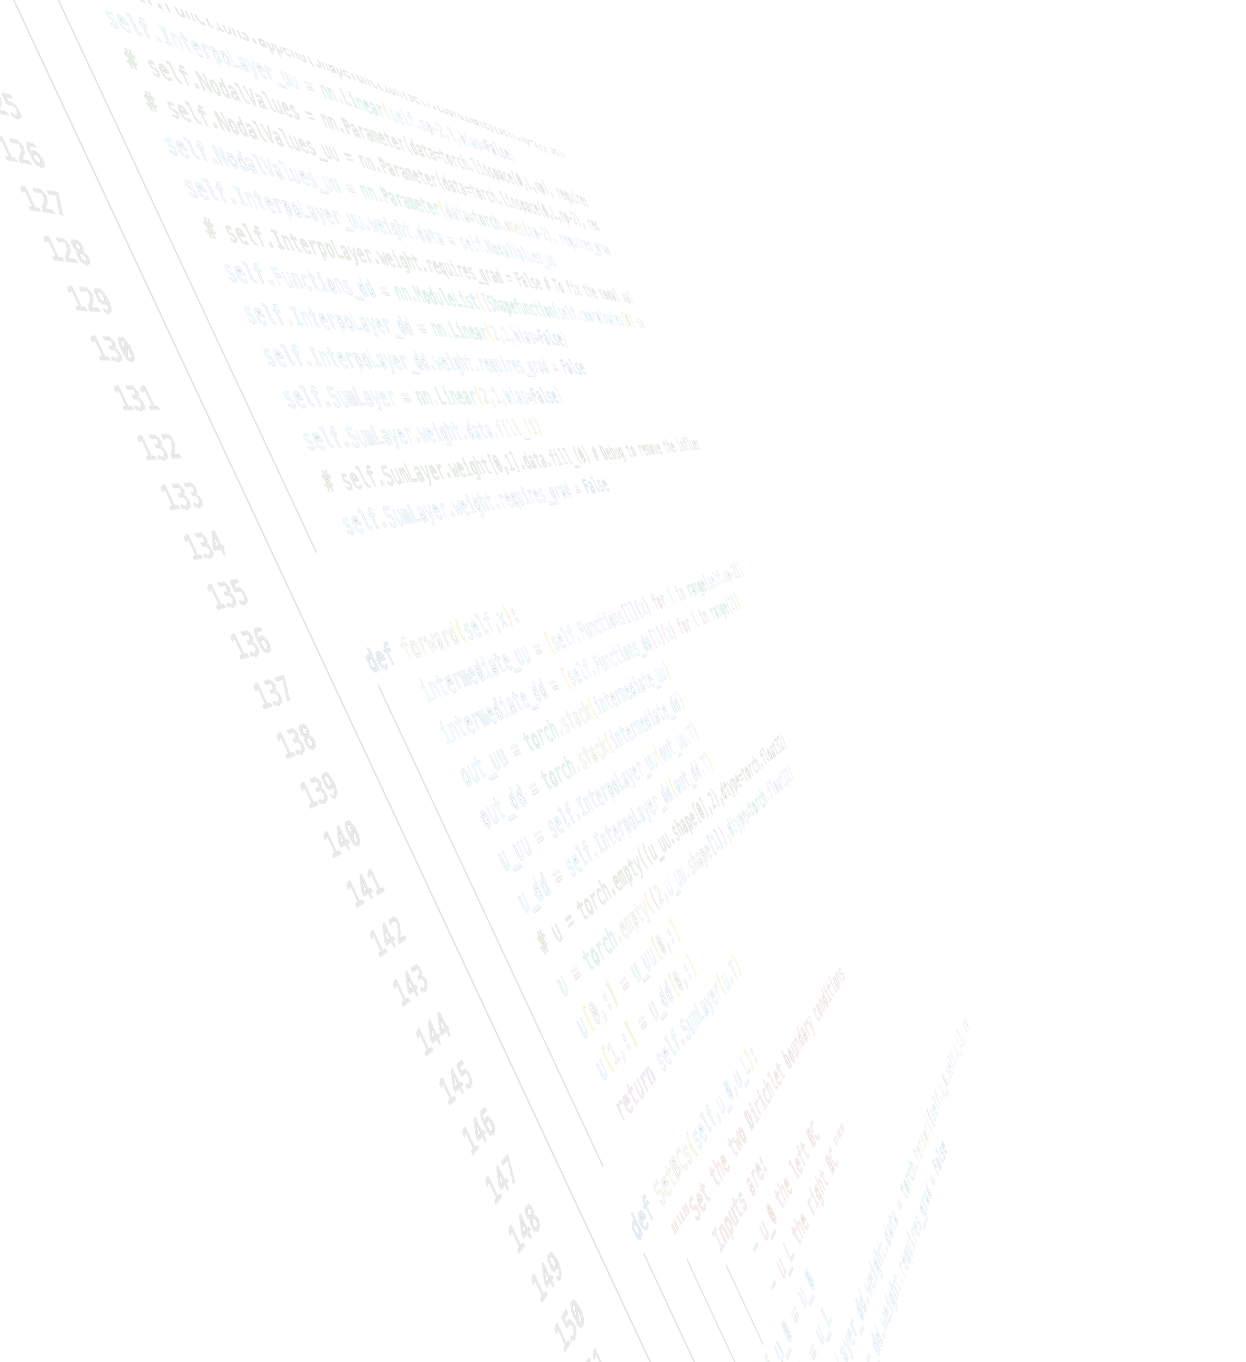
\includegraphics[width=\imagewidth]{Logos/LMS/Code_light.png}
			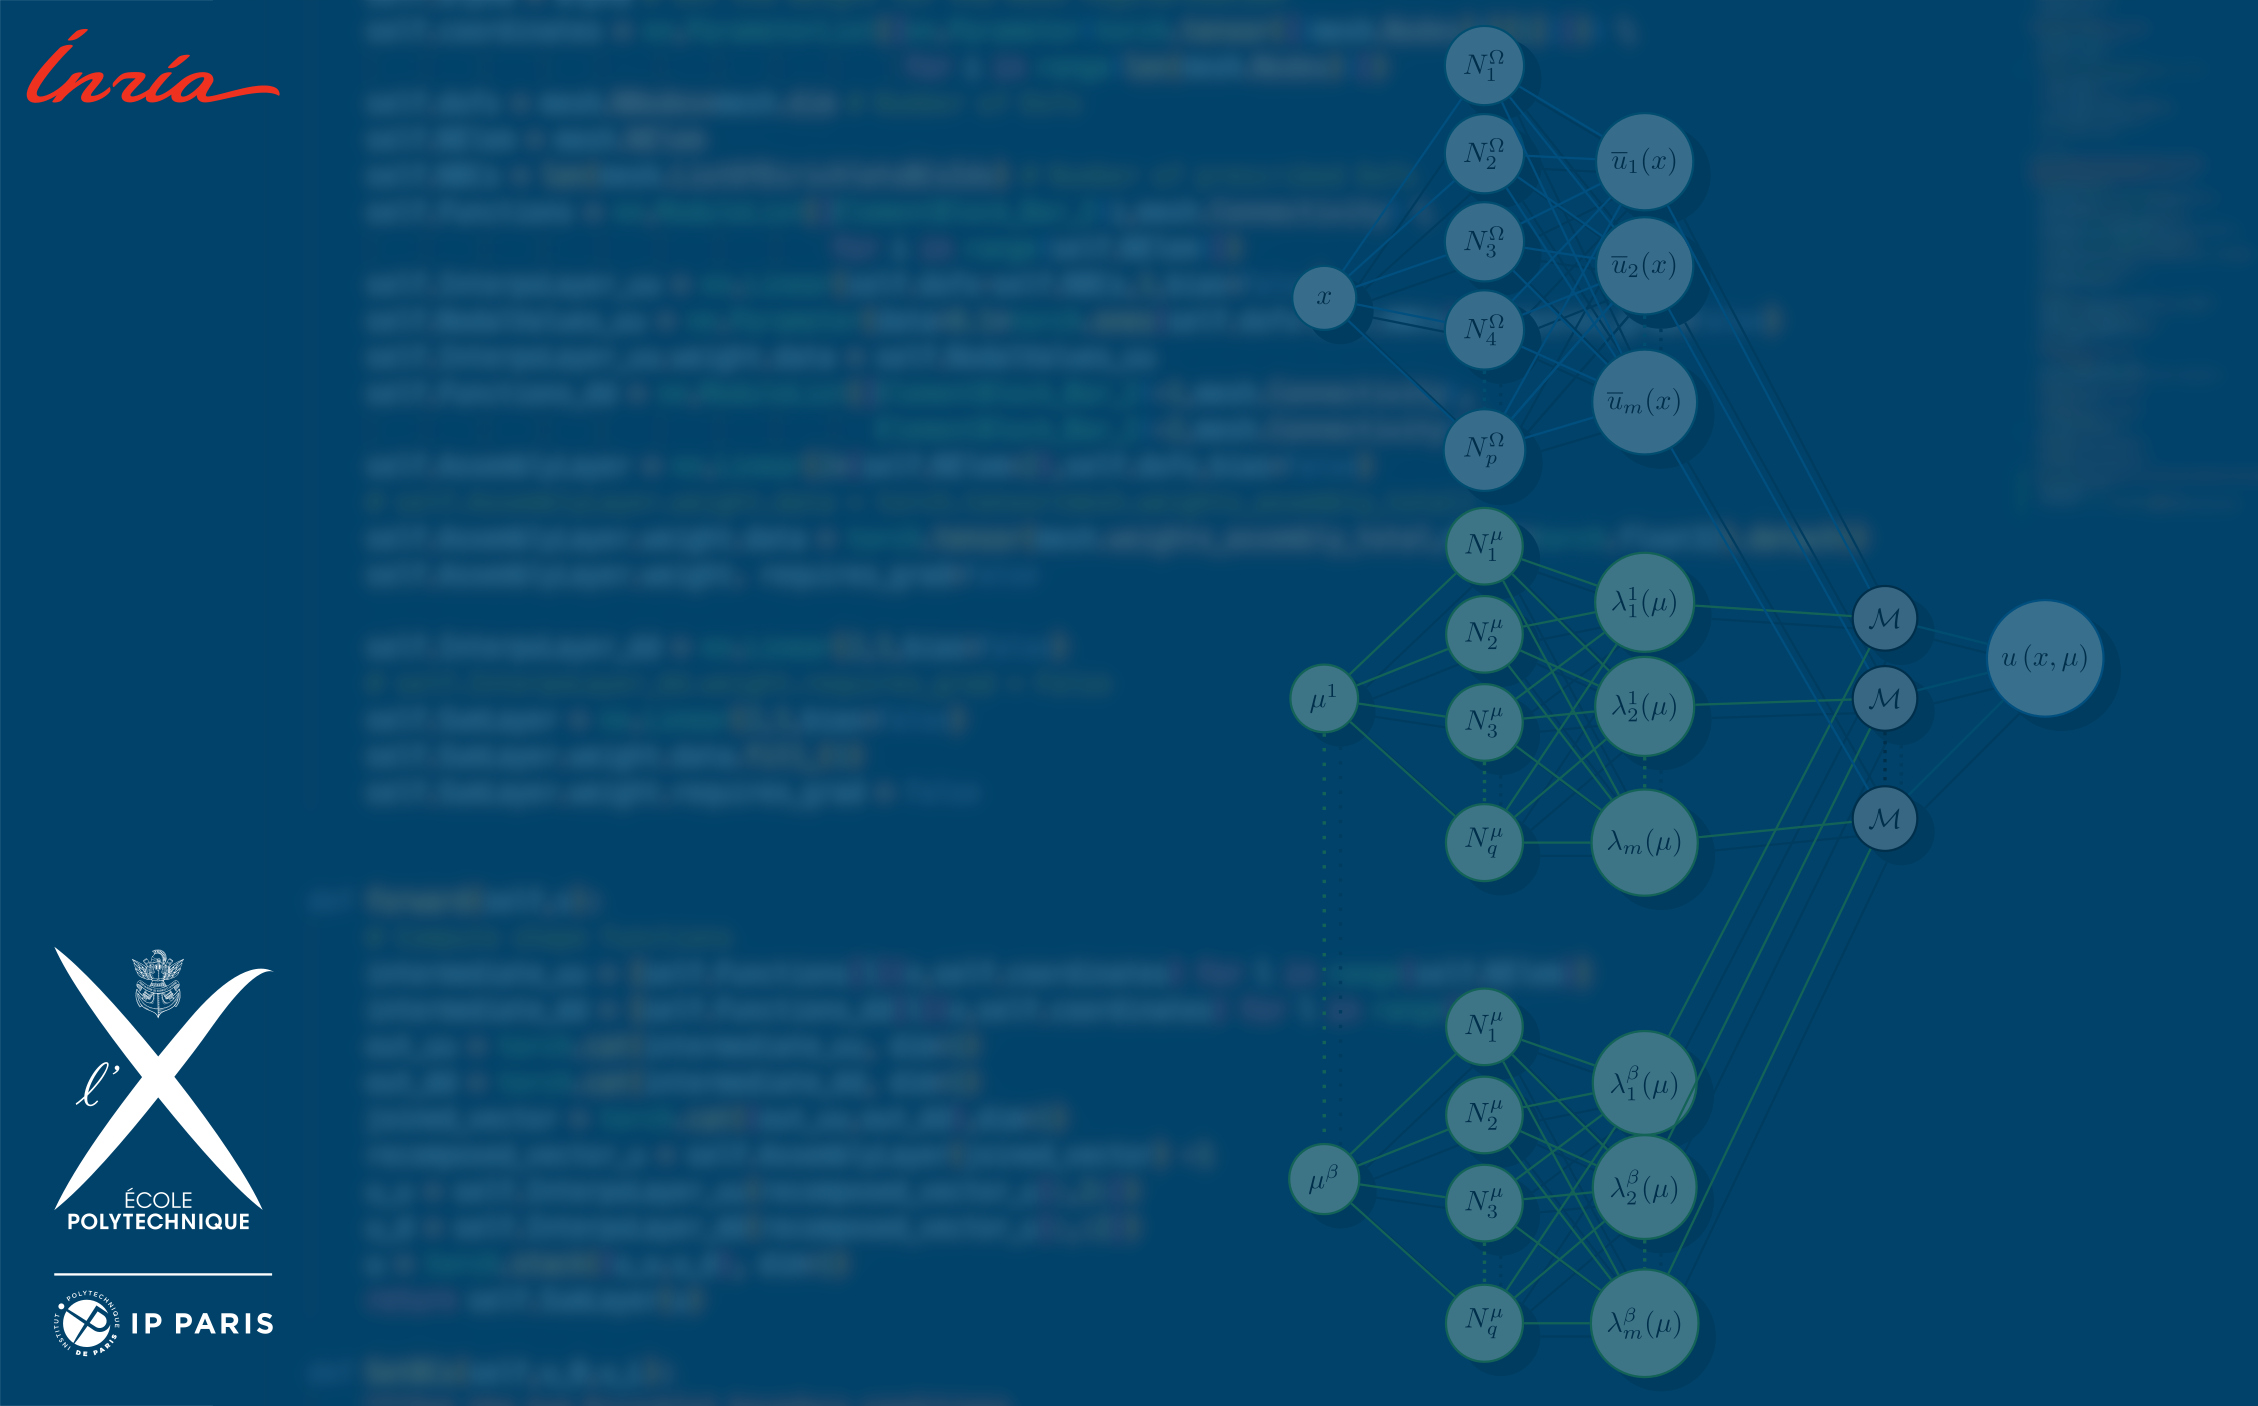
\includegraphics[width=1.121\imagewidth]{Logos/LMS/TitlePage.png}
			}
			\frame[plain]{\titlepage} 
		}
	%---------------------------------------------------------
	\section{Scientific background}
        \subsection{Project}
	\begin{frame}
		\frametitle{\textsc{Scientific project}}
		\framesubtitle{Computational mechanics} 
		\begin{blueblockshadow}{Objectives:}
				\begin{itemize}
					\item Transfer the tools to the clinic
					\item Easy access to a patient specific model of the lungs
					\begin{itemize}
						\item Parameters estimation (inverse problem) on the fly 
						\item Real time computations
					\end{itemize}
					\item Physics-coherent solutions
				\end{itemize}
		\end{blueblockshadow}
		\vfill
		\begin{minipage}[t]{0.5\linewidth}
			\begin{greenblockshadow}{Scientific context}
				\begin{itemize}
%					\item[\textcolor{LGreenLMS}{\faCheckSquare}] Reliable model of the lung
					\item[\textcolor{LGreenLMS}{\faLockOpen}] Reliable model of the lung
					\begin{itemize}
						\item Macro \& micro scales
					\end{itemize}
					\item[{\textcolor{RougeLMS}\faLock}] Efficient computational strategy 
					\begin{itemize}
						\item Rapid estimation of patient-specific parameters 
						\item Micro-scale model at the structure scale 
					\end{itemize}
				\end{itemize}
			\end{greenblockshadow}
		\end{minipage}
		\hfill
		\begin{minipage}[t]{0.48\linewidth}
			\begin{greenblockshadow}{Proposed numerical strategy}
				\begin{itemize}
					\item Reduced-order modelling $\vect{u} = \vect{u}\left(\vect{x},t,\vect{\mu}\right)$
					\begin{itemize}
						\item[\textcolor{GreenLMS}{\faCogs}] HiDeNN, Reduced-order bases, etc.
					\end{itemize}
					\item Robust and flexible methodology
					\begin{itemize}
						\item Modular approach, keep each step separated
					\end{itemize}
				\end{itemize}
			\end{greenblockshadow}
		\end{minipage}
	\end{frame}
\subsection{Litterature }
\begin{frame}
    \frametitle{\textsc{Scientific project}}
    \framesubtitle{Surrogate and reduced-order modelling } 
    \begin{itemize}
        \item ML based surrogate models
        \begin{itemize}
            \item Purely data driven methods
            \begin{itemize}
                \item[{\footnotesize \color{LGreenLMS} \faPlusSquare}] Approximation of highly nonlinear systems
                \item[{\footnotesize \color{RougeLMS} \faMinusSquare}] Dependence on architecture 
                \item[{\footnotesize \color{RougeLMS} \faMinusSquare}] Low interoperability
            \end{itemize}
            \item Physics-informed neural networks
            \begin{itemize}
                \item[{\footnotesize \color{LGreenLMS} \faPlusSquare}] Loss function based residuals for governing equations
                \item[{\footnotesize \color{RougeLMS} \faMinusSquare}] Dependence on architecture 
            \end{itemize}
            \item Hierarchical deep-learning neural networks (HiDeNN)
            \begin{itemize}
                \item[{\footnotesize \color{LGreenLMS} \faPlusSquare}] Loss function based residuals for governing equations
                \item[{\footnotesize \color{LGreenLMS} \faPlusSquare}] Architecture based on domain disretization
                \item[{\footnotesize \color{RougeLMS} \faMinusSquare}] Neumann boundary conditions not strongly prescribed, yet
            \end{itemize}
        \end{itemize}
        \item Classical reduced-order models
        \begin{itemize}
            \item \emph{A posteriori}: POD 
            \begin{itemize}
                \item[{\footnotesize \color{LGreenLMS} \faPlusSquare}] Works well with standard non-linear solvers (Newton-Raphson, Arc-length, etc.)
                \item[{\footnotesize \color{RougeLMS} \faMinusSquare}] Requires well-suited previous expensive computations
                \item[{\footnotesize \color{RougeLMS} \faMinusSquare}] Requires guessing the required reduced-order basis size
            \end{itemize}
            \item \emph{A priori}: PGD
            \begin{itemize}
                \item[{\footnotesize \color{LGreenLMS} \faPlusSquare}] Reduced-order basis built and adapted on the fly
                \item[{\footnotesize \color{RougeLMS} \faMinusSquare}] Requires space-time linearisation of the problem
                \item[{\footnotesize \color{RougeLMS} \faMinusSquare}] Not well suited to large number of parameters
            \end{itemize}
        \end{itemize}
    \end{itemize}
\end{frame}


\section{Machine learning \& computational mechanics}
\subsection{PINNs}
 \begin{frame}
    %\frametitle{\textsc{ML-based model reduction}}
    %\framesubtitle{Physics-informed neural networks} 
    \frametitle{\textsc{Physics-informed neural networks}}

    \begin{columns}
    \begin{column}{0.6\textwidth}
    
    \begin{blueblockshadow}{Test problem setting}
    \begin{columns}
    \begin{column}{0.6\textwidth}
    \scriptsize{
    \begin{align*}
	\underline{\mathrm{div}}  (\doubleunderline{ \sigma})  &= 0 \qquad \mathrm{on} \ \Omega \\
	\doubleunderline{ \sigma} \cdot \underline{n} &= 0 \qquad \mathrm{on} \ \Gamma_{N_0} \\
	\doubleunderline{ \sigma} \cdot \underline{n} &= \underline{g} \qquad \mathrm{on} \ \Gamma_{N_1} \\
        \underline{u} &= u_D \qquad \mathrm{on} \  \Gamma_ D\\
	\mathrm{where} \quad \doubleunderline{ \sigma} &= \doubleunderline{C}:\epsilon(u)
    \end{align*}}
    \end{column}
    \begin{column}{0.4\textwidth}
        \begin{figure}
        \centering
        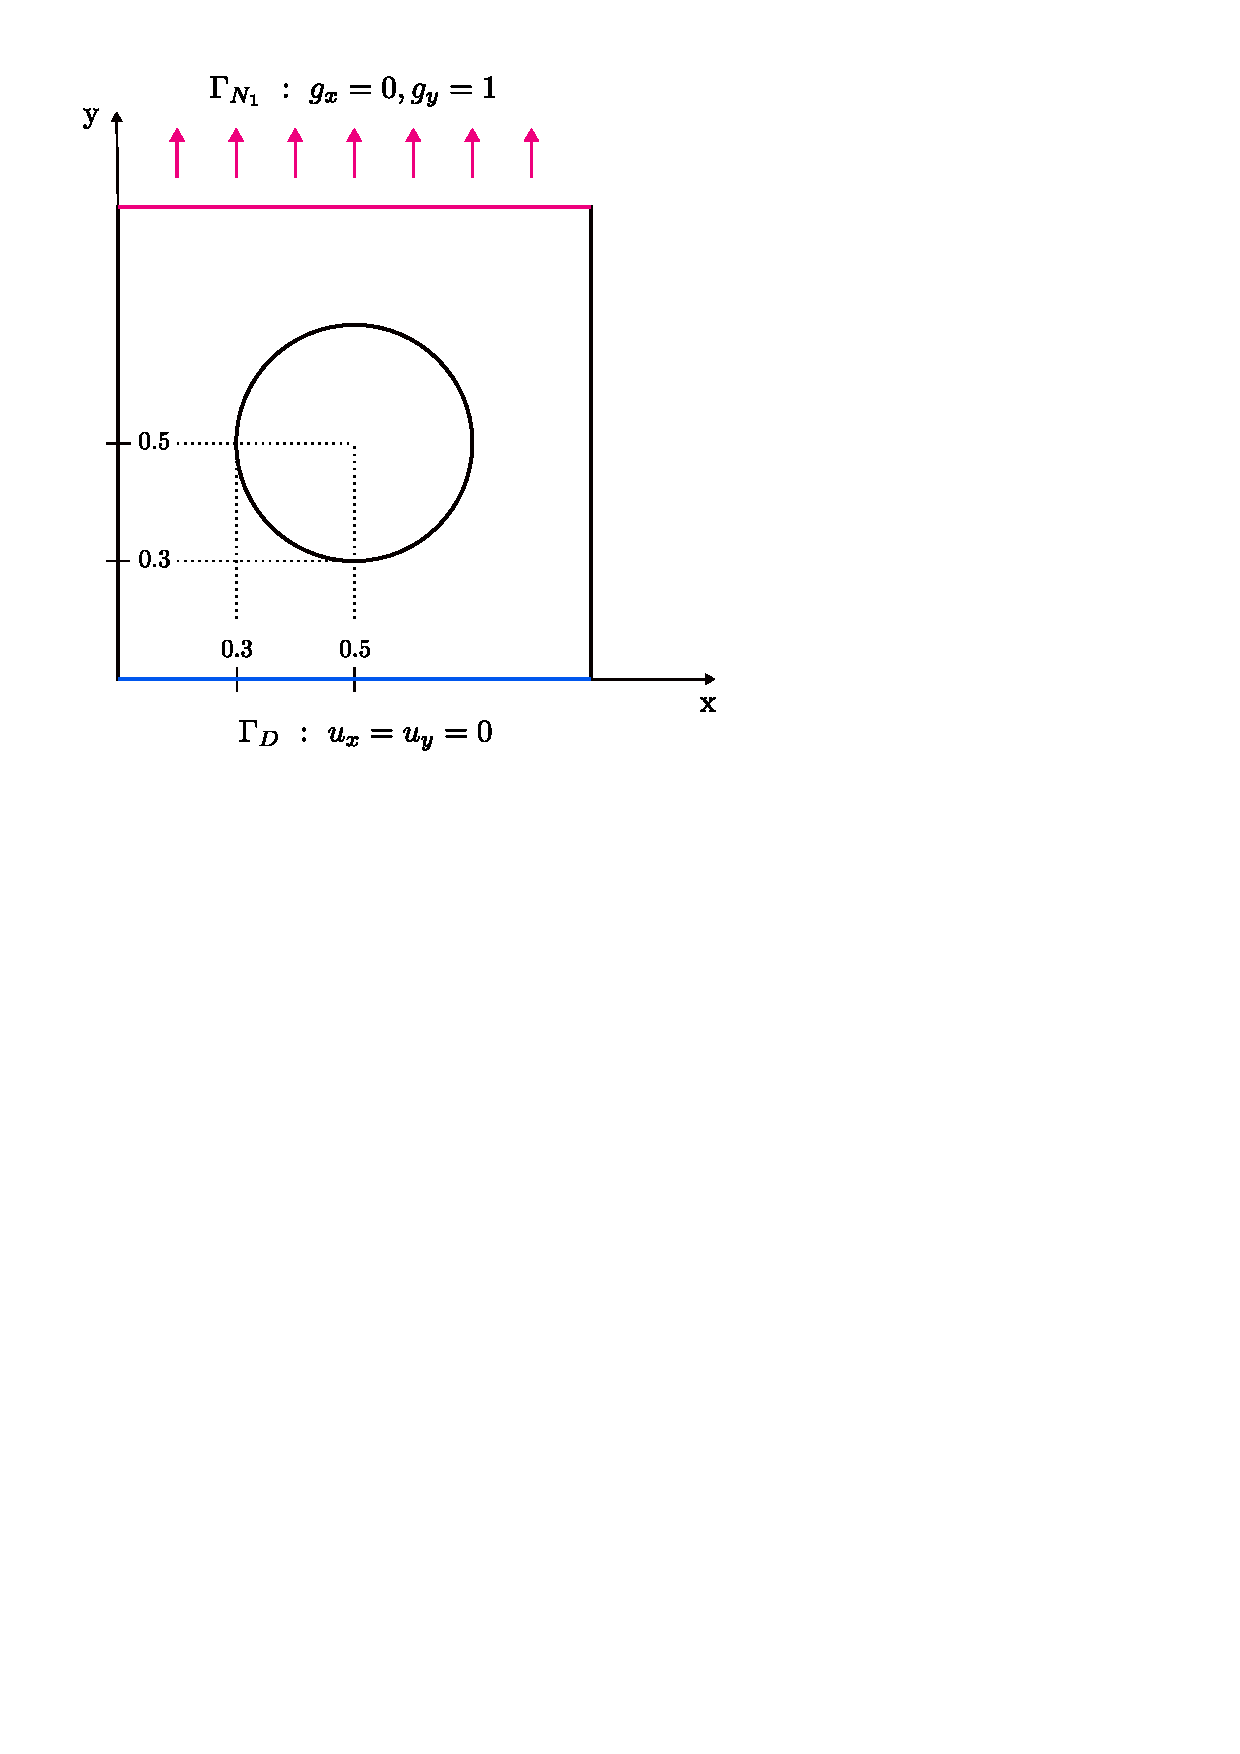
\includegraphics[trim={0 17cm 8cm 1cm},clip,width = 0.95\linewidth]{Figures/PINN_problem_1.pdf}    
        \end{figure}
    \end{column}
    \end{columns}
    \end{blueblockshadow}

    \vspace{0.3cm}

    \begin{blueblockshadow}{PINN formulation}
    \scriptsize{
        \begin{align*}
            \mathcal{L} &= \mathcal{L}_{\mathrm{PDE}} + \mathcal{L}_{\mathrm{BC_N}}+ \mathcal{L}_{\mathrm{BC_D}}+ \mathcal{L}_{\mathrm{Constit}}\\
            \mathcal{L}_{\mathrm{PDE}} &=  \frac{1}{N_i}\sum_{i=0}^{N_i} \left(\underline{\mathrm{div}}  (\doubleunderline{ \sigma}(x_i)\right)^2 \\
            \mathcal{L}_{\mathrm{PDE}} &=  \frac{1}{N_i}\sum_{i=0}^{N_i} \left((\doubleunderline{ \sigma}(x_i) - (\doubleunderline{ \hat{\sigma}}(\underline{u}(x_i)\right)^2
        \end{align*}}
    \end{blueblockshadow}
    \end{column}
    \begin{column}{0.33\textwidth}

        \begin{figure}
        \centering
        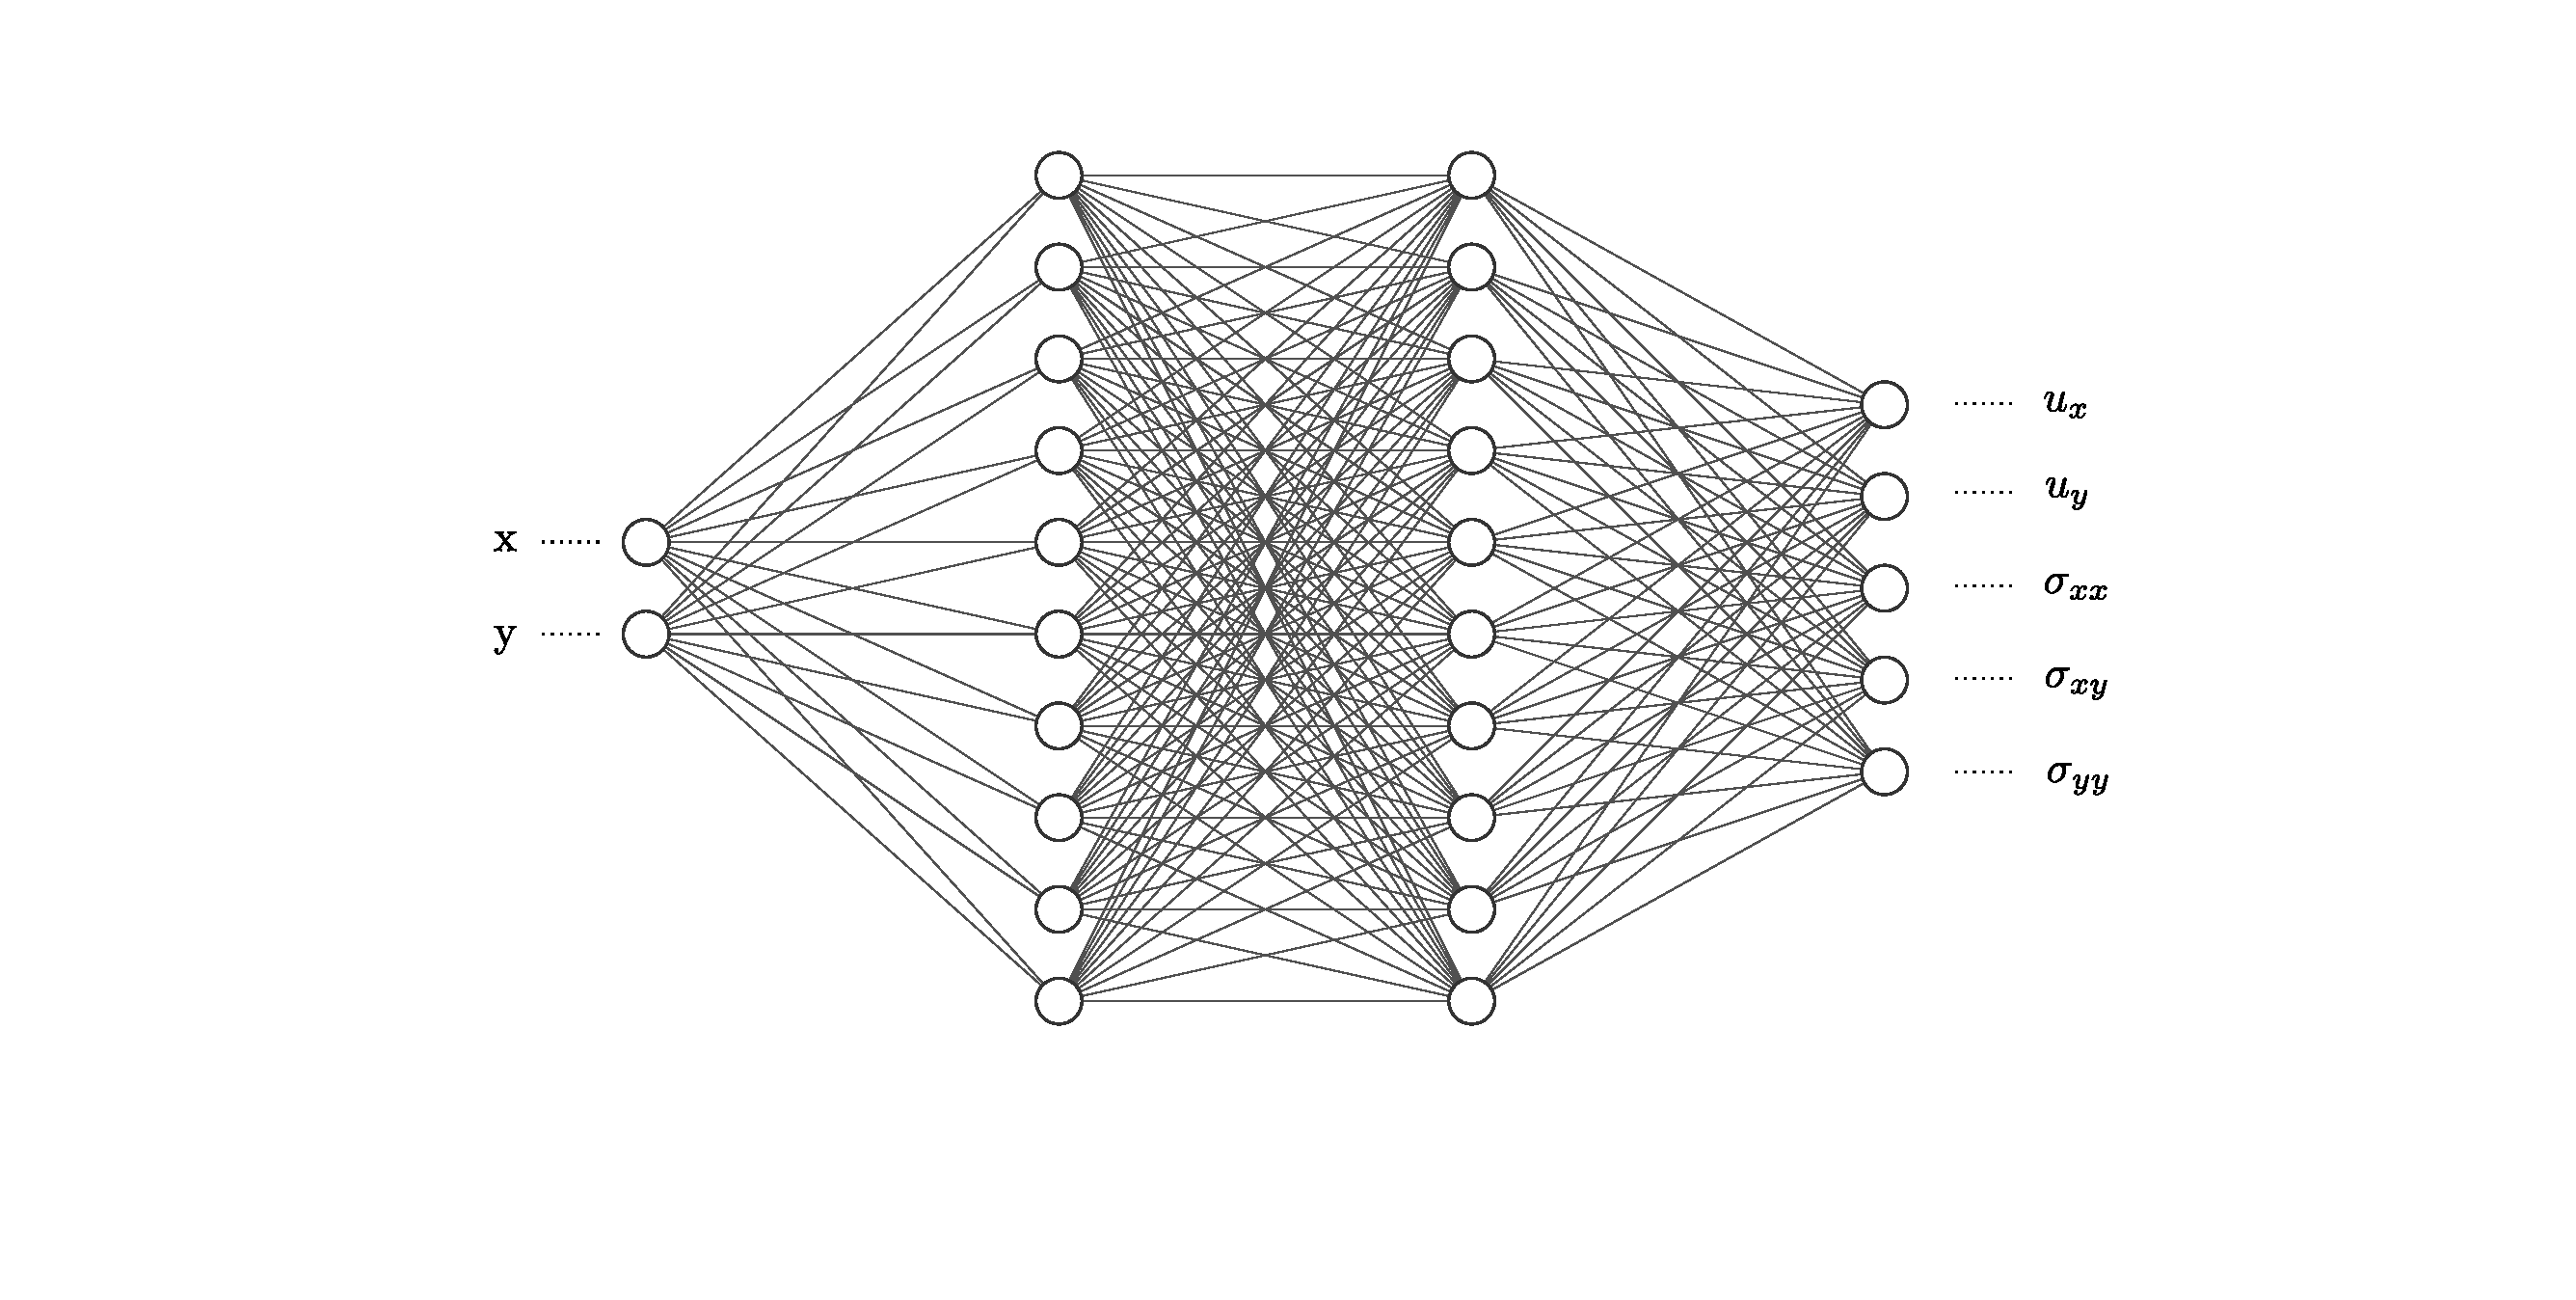
\includegraphics[trim={8cm 2cm 8cm 2.5cm},clip,width = 0.98\linewidth]{Figures/PINN_arch1.pdf}    
        \end{figure}
        \begin{figure}
        \centering
        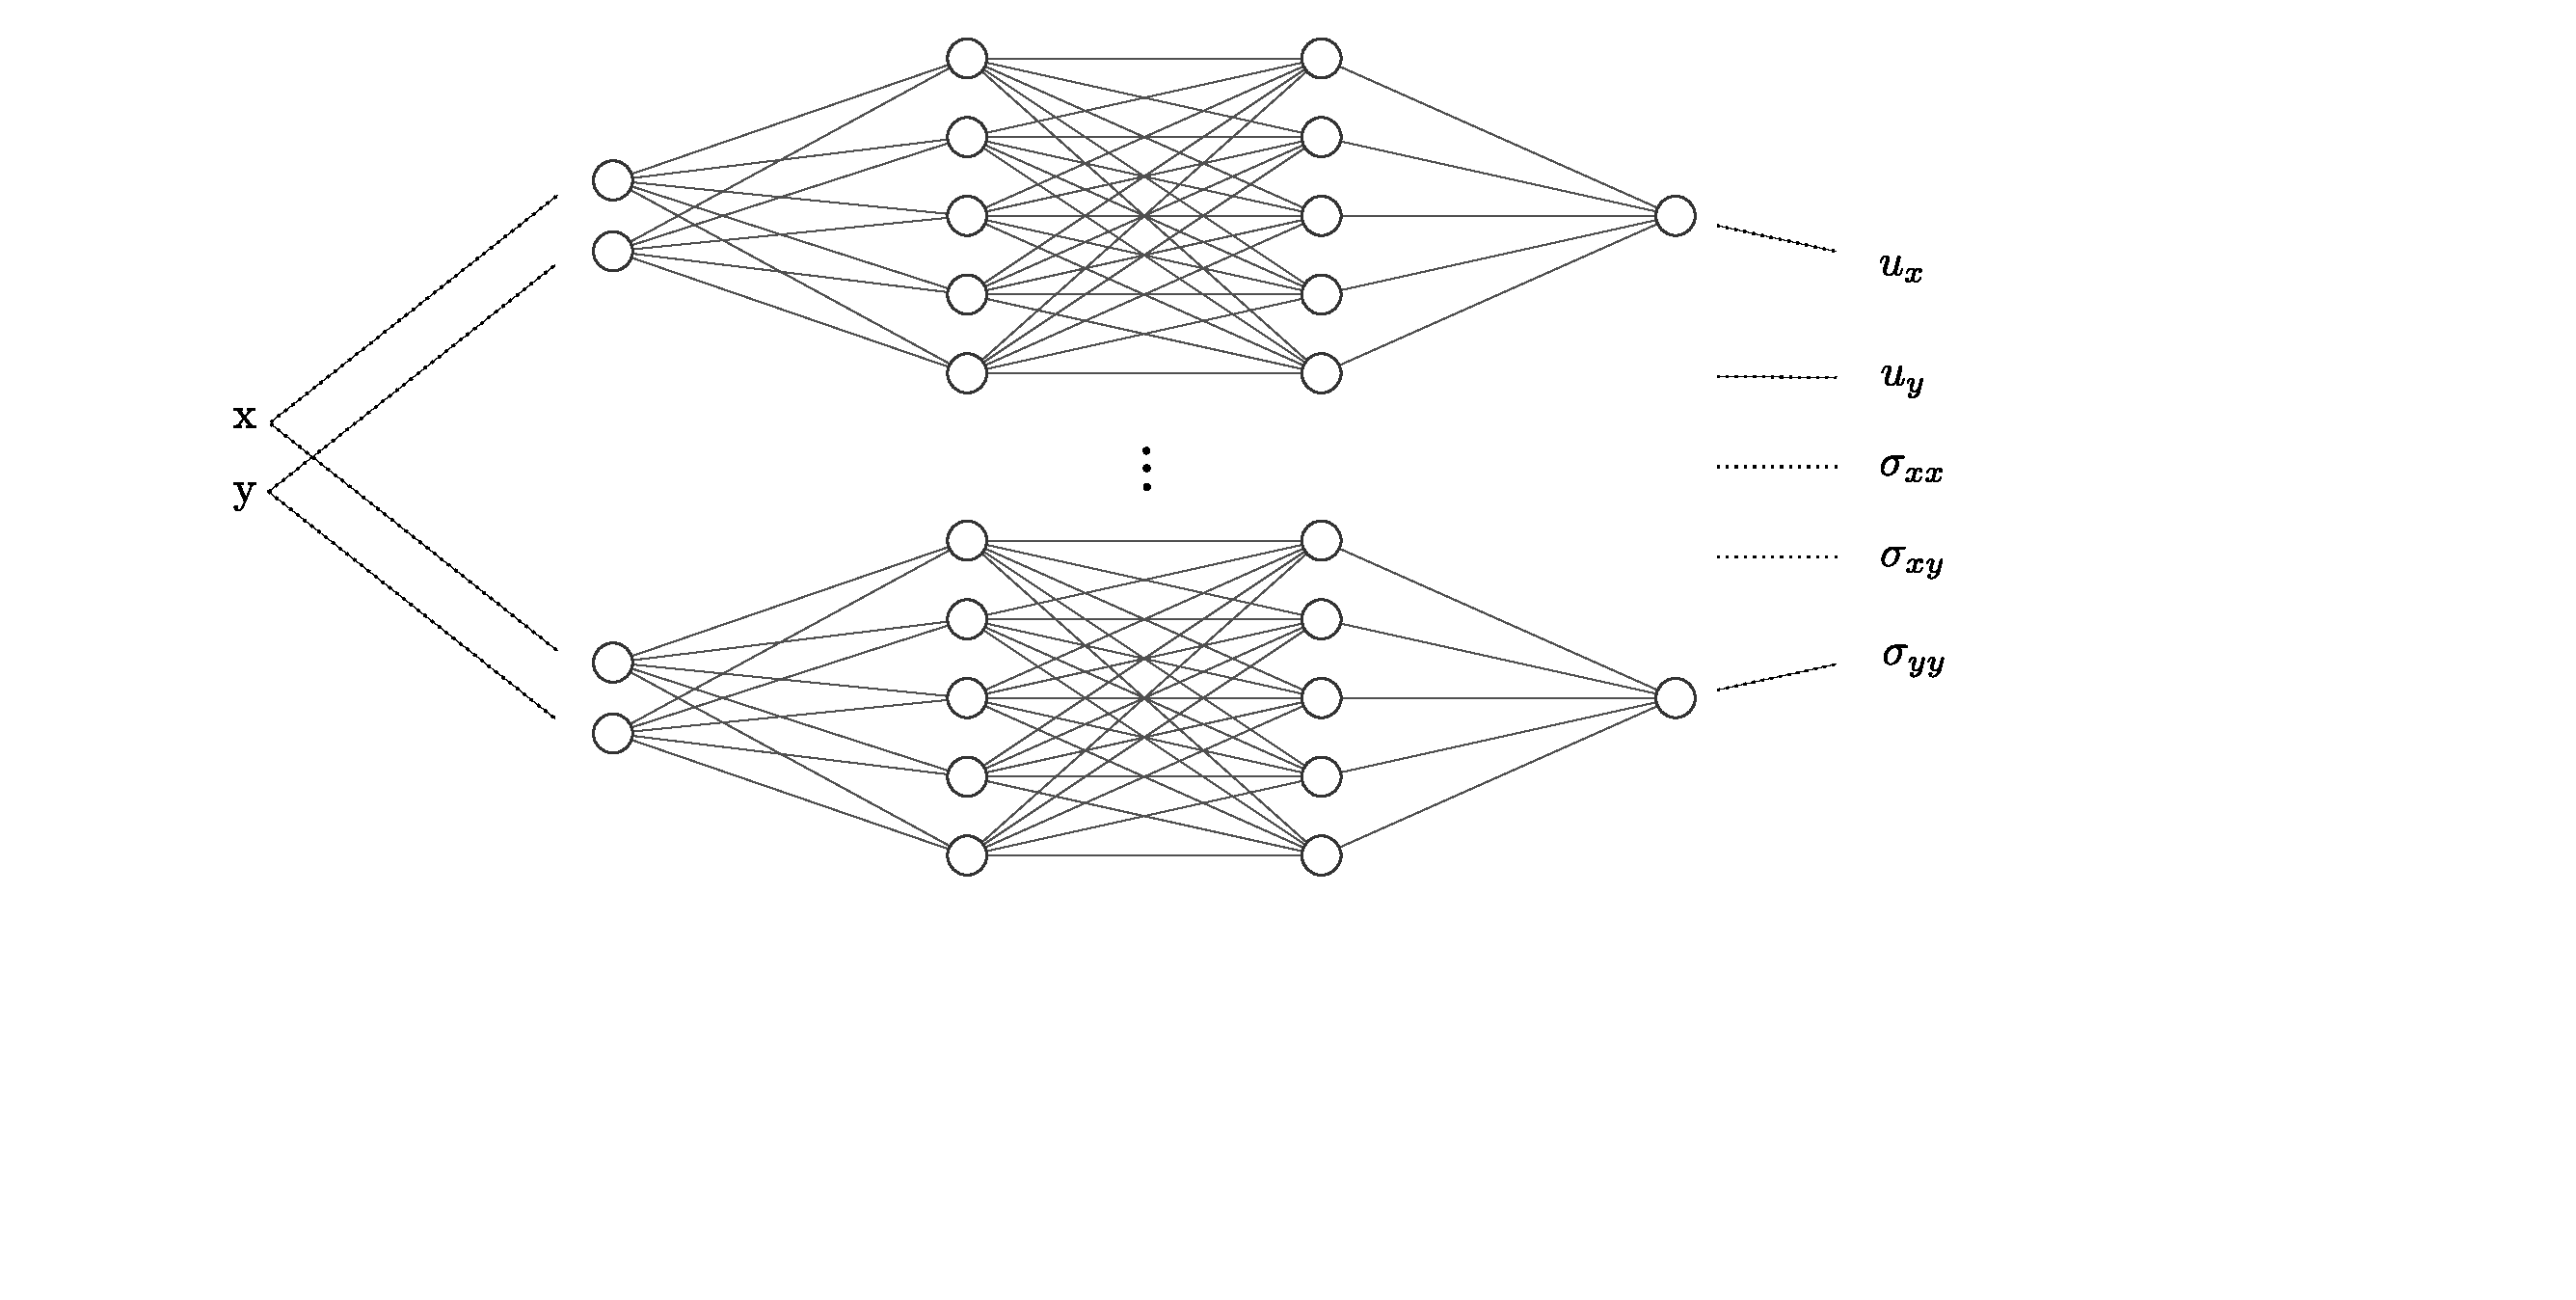
\includegraphics[trim={4cm 2cm 11cm 0cm},clip,width = 0.98\linewidth]{Figures/PINN_arch2.pdf}    
        \end{figure}

    \end{column}
    \end{columns}   
 \end{frame}

\begin{frame}
    %\frametitle{\textsc{ML-based model reduction}}
    %\framesubtitle{Physics-informed neural networks} 
    \frametitle{\textsc{Physics-informed neural networks}}

    \begin{columns}
    \begin{column}{0.48\textwidth}
    
    \begin{blueblockshadow}{Parameters of PINNs \& Training}
    \vspace{0.2cm}
    \begin{itemize}
        \item[{\fontfamily{cyklop}\selectfont \footnotesize{?}}] 1 PINN vs. multiple PINNs
        \item[{\fontfamily{cyklop}\selectfont \footnotesize{?}}] Number of hidden layers
        \item[{\fontfamily{cyklop}\selectfont \footnotesize{?}}] Number of nodes in each layer
        \item[{\fontfamily{cyklop}\selectfont \footnotesize{?}}] Activation function
        \item[{\fontfamily{cyklop}\selectfont \footnotesize{?}}] Optimiser + learning rate
        \item[{\fontfamily{cyklop}\selectfont \footnotesize{?}}] Composition of training data 
        \begin{itemize}
            \item Interior points
            \item Boundary points
        \end{itemize}
    \end{itemize}
    \end{blueblockshadow}
    \end{column}
    \begin{column}{0.48\textwidth}
    
    \begin{figure}
     \centering
     \begin{subfigure}[b]{0.4\textwidth}
         \centering
         \includegraphics[trim={14cm 5cm 16cm 7cm},clip,width = \textwidth]{Figures/PINN_u_1.pdf}
         \caption{$u_x$}
     \end{subfigure}
     \begin{subfigure}[b]{0.4\textwidth}
         \centering
         \includegraphics[trim={14cm 5cm 16cm 7cm},clip,width = \textwidth]{Figures/PINN_u_error_1.pdf}
        \caption{$u_x^{FEM} - u_x$}
     \end{subfigure}\\
     \begin{subfigure}[b]{0.4\textwidth}
         \centering
         \includegraphics[trim={14cm 5cm 16cm 7cm},clip,width = \textwidth]{Figures/PINN_v_1.pdf}
        \caption{$u_y$}
     \end{subfigure}
     \begin{subfigure}[b]{0.4\textwidth}
         \centering
         \includegraphics[trim={15.5cm 5cm 15.5cm 7cm},clip,width = \textwidth]{Figures/PINN_v_error_1.pdf}
        \caption{$u_y^{FEM} - u_y$}
     \end{subfigure}
         \caption{\scriptsize{4 $\times$ 96 nodes ($38021$ trainable parameters)}}
     \end{figure}
    \end{column}
    \end{columns} 


    \begin{blueblockshadow}{Conclusions}
    \begin{itemize}
        \item Relative error w.r.t FEM solution $\geq 10\%$ for $u_x, \sigma_{xx}, \sigma_{xy}$
        \item Boundary conditions not strongly presribed
        \item The optimal architecture and learning strategy is strongly problem-dependent
    \end{itemize}
    \end{blueblockshadow}
\end{frame}
\subsection{HiDeNN}
    \begin{frame}{\textsc{Hierarchical Deep Neural Network}}
    \framesubtitle{Interpretable neural network}
        \begin{blueblockshadow}{HiDeNN}
        \begin{itemize}
            \item Non-fully connected layers
            \begin{itemize}
                \item Fewer parameters to train
            \end{itemize}
            \item Reproducing the interpolation of a Finite Element mesh
            \begin{itemize}
                \item Understand the role and impact of each parameter
                \item Possibility to refine and change the architecture without loosing the previous training
            \end{itemize}
        \end{itemize}
        \end{blueblockshadow}
        \vfill
        \begin{greenblockshadow}{\textsc{Parametric use}}
            \begin{itemize}
                \item Rely on the architecture to perform interpolation in the parametric domain
                \begin{itemize}
                    \item Extends the above-mentioned benefits to the parameter space
                \end{itemize}
                \item Include on a tensor decomposition (ROM)
                \begin{itemize}
                    \item Retrieve the standard benefits of ROM
                    \item Get a fully parameterised model to use in real time after training
                \end{itemize}
            \end{itemize}
        \end{greenblockshadow}
    \end{frame}

    \begin{frame}
        \frametitle{\textsc{Spatial representation of the parameters}}
        \framesubtitle{HiDeNN-PGD}
        \begin{minipage}{0.58\linewidth}
    
                \begin{itemize}
                    \item For a new patient, get a map of the parameter field $\mu\left(x\right)$ through segmentation
                    \item Project $\mu\left(x\right)$ onto a basis $\left\{f^k\left(x\right)\right\}_{k \in \llbracket 1, \beta \rrbracket}$
                    \begin{itemize}
                        \item $\mu\left(x\right) = \sum\limits_{k=1}^{\beta}\mu^{k}f^k\left(x\right)$
                        \item $\left\{u^k\right\}_{k \in \llbracket 1, \beta \rrbracket}$ input parameters for the NN
                    \end{itemize}
                    \item \small{$\displaystyle\vect{u}(\textcolor{BleuLMS!70}{\vect{x}},\textcolor{LGreenLMS}{\vect{\mu^1}, \cdots, \vect{\mu}^{\beta}}) = \sum\limits_{i=1}^m \textcolor{BleuLMS!70}{\overline{\vect{u}}_i(\vect{x})} ~\textcolor{LGreenLMS}{\prod_{j=1}^{\beta}\lambda_i^j(\vect{\mu^j})}$} 
                    \item Retrieve $\mu\left(x\right)$ for computing the physical loss 
                    \begin{itemize}
                        \item $\mathcal{L} = g\left(\vect{u}\left(\textcolor{BleuLMS!70}{\vect{x}},\textcolor{LGreenLMS}{\left\{\mu^k\right\}}\right),\textcolor{BleuLMS!70}{\vect{x}},\mu\left(x\right)\right) $
                    \end{itemize}
                    \item[\textcolor{LGreenLMS}{\faLockOpen}] Non-linear interpolation using \emph{a priori} ROM 
                    \begin{itemize}
                        \item By adding an intermediate layer between the modes and the interpolated result
                    \end{itemize}
                    \item[\textcolor{LGreenLMS}{\faLockOpen}] Is not fixed for a given parameter discretisation
                        \begin{itemize}
                            \item Mesh less method
                        \end{itemize}
                \end{itemize}
    
        \end{minipage}
        \hfill 
        \begin{minipage}{0.38\linewidth}
            \centering
    
            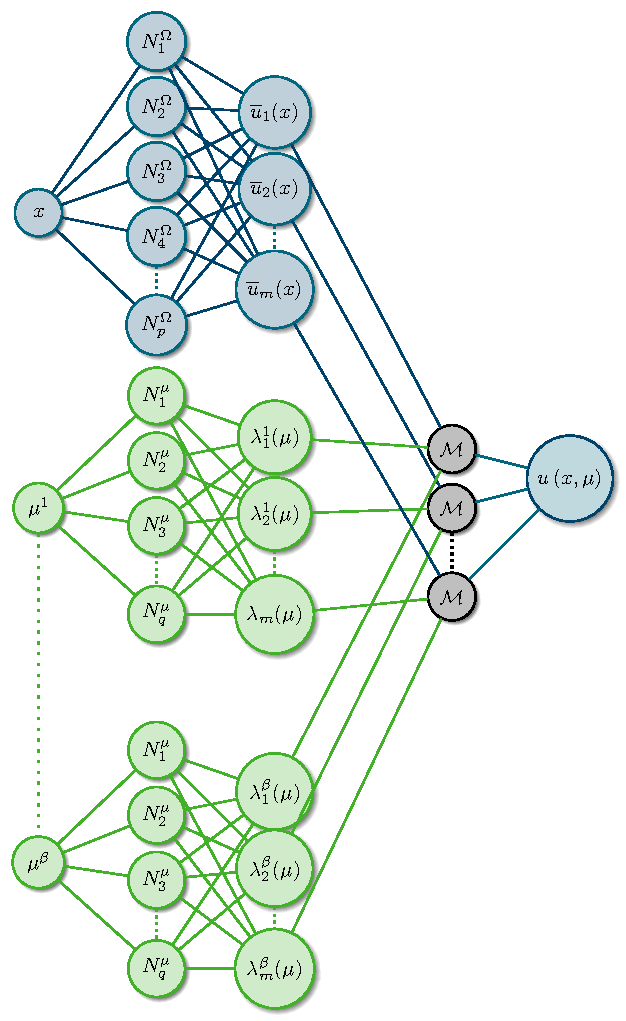
\includegraphics[width=\linewidth]{Schema/HiDeNN-TD-SpatialParam.pdf}
        \end{minipage}
    \end{frame}
\section{Perspectives}
    \begin{frame}{\textsc{Perspectives - 2024}}
    \framesubtitle{Project schedule}
        \vspace{-5pt}
        \begin{center}
            		\centering
		% \begin{ganttchart}[
		% 	hgrid,
		% 	vgrid,
		% 	x unit=1cm,
		% 	y unit chart=0.5cm,
		% 	title height=1,
		% 	title label font=\bfseries\footnotesize,
		% 	bar/.style={draw, fill=BleuLMS},
		% 	bar height=0.7,
		% 	bar label font=\small,
		% 	group right shift=0,
		% 	group top shift=0.5,
		% 	group height=0.3,
		% 	group peaks width=0.2,
		% 	inline
		% 	]{1}{11}
		% 	% \gantttitle{2024 Schedule}{11} \\
		% 	\gantttitlelist{2,...,12}{1} \\
		% 	\ganttbar[bar/.append style={fill=GreenLMS}]{\color{white}Method paper 1}{1}{5} \\
		% 	\ganttbar{\color{white}Method paper 2}{1}{5} \\
		% 	\ganttnewline
		% 	\ganttmilestone{Tools}{5} \ganttnewline
		% 	\ganttnewline
		% 	\ganttbar{\color{white}Application paper 1}{6}{11} \\
		% 	\ganttbar[bar/.append style={fill=GreenLMS}]{\color{white}Application paper 2}{6}{11} \\
		% 	% \ganttgroup[group/.append style={fill=BleuLMS!20!black}]{Phase 1}{1}{5} \\
		% 	% \ganttgroup[group/.append style={fill=BleuLMS!20!black}]{Phase 2}{6}{11} \\
		% 	\ganttlink{elem0}{elem2}
		% 	\ganttlink{elem1}{elem2}
		% 	\ganttlink{elem2}{elem3}
		% 	\ganttlink{elem2}{elem4}
		% \end{ganttchart}

\begin{ganttchart}[
        hgrid,
	vgrid,
	x unit=1cm,
	y unit chart=0.5cm,
	today=1,
	progress=today,
	title height=1,
	title label font=\bfseries\footnotesize,
	bar/.style={draw, fill=BleuLMS!20},
	bar incomplete/.append style={fill=BleuLMS},
	bar height=0.7,
	bar label font=\small,
	group right shift=0,
	group top shift=0.5,
	group height=0.3,
	group peaks width=0.2,
	inline
	]{1}{12}
	% \gantttitle{2024 Schedule}{11} \\
	\gantttitlelist{1,...,12}{1} \\
	\ganttbar[progress label text={},bar/.append style={fill=GreenLMS!20},bar incomplete/.append style={fill=GreenLMS}]{\color{white}Method paper 1}{1}{5} \\
	\ganttbar[progress label text={}]{\color{white}Method paper 2}{2}{5} \\
	\ganttnewline
	\ganttmilestone[progress label text={}]{Tools}{5} \ganttnewline
	\ganttnewline
	\ganttbar[progress label text={},bar/.append style={fill=GreenLMS!20},bar incomplete/.append style={fill=GreenLMS}]{\color{white}Application paper 1}{6}{12} \\
	\ganttbar[progress label text={}]{\color{white}Application paper 2}{6}{12} \\
	% \ganttgroup[group/.append style={fill=BleuLMS!20!black}]{Phase 1}{1}{5} \\
	% \ganttgroup[group/.append style={fill=BleuLMS!20!black}]{Phase 2}{6}{11} \\
	\ganttlink{elem0}{elem2}
	\ganttlink{elem1}{elem2}
	\ganttlink{elem2}{elem3}
	\ganttlink{elem2}{elem4}
\end{ganttchart}
  

        \end{center}
        \vspace{-10pt}
        \begin{greenblockshadow}{Detail}
            \begin{minipage}{0.48\linewidth}
                \begin{itemize}
                \item Method papers
                \begin{itemize}
                    \item PDE focused (Mixed formulation, Training strategy, etc.)
                    \item Parametric surrogate modelling (ROM, Space parameter fields)
                \end{itemize}
                \end{itemize}
            \end{minipage}
            \hfill\vline\hfill
            \begin{minipage}{0.48\linewidth}
                \begin{itemize}
                \item Application papers
                \begin{itemize}
                    \item Application to the micro-model
                    \item Application to the macro-model
                \end{itemize}
                \end{itemize}
            \end{minipage}
        \end{greenblockshadow}
    \end{frame}
 \end{document}